\documentclass[a4paper,12pt]{article}
\usepackage[a4paper,margin=1in,footskip=0.25in]{geometry}
\usepackage[utf8]{inputenc}

% science
\usepackage{amsmath}
\usepackage{array}
\usepackage{siunitx}

% layout
\usepackage{float}
\usepackage{parskip}
\usepackage{graphicx}
\usepackage{circuitikz}
\usepackage{longtable}
\usepackage{hyperref}


% referencing
\usepackage[style=apa]{biblatex}
\addbibresource{light.bib}
\usepackage{hyperref}

% table centering
\renewcommand{\arraystretch}{1.3}
\newcolumntype{P}[1]{>{\raggedright\arraybackslash}p{#1}}
\newcommand{\tptt}{$\times\,$}

% figures labelings
\usepackage{chngcntr}
\counterwithin{figure}{section}

% uncertainty
\newcommand{\absun}{\Delta \text{unc}\,}
\newcommand{\relun}{\% \text{unc}\,}
\newcommand{\tsf}{\,\text{sf}}

\newcommand{\paragraphnl}[1]{\textbf{#1}\\\\}

\usepackage{caption}
\usepackage{subcaption}
\usepackage{wrapfig}

\title{Empirically finding the typical luminous efficacy of an incandescent light-bulb through the inverse square law}

% no author or date
\author{}
\date{\vspace{-8ex}}

\begin{document}

\maketitle

\section{Design}

\subsection{Introduction}
I watched a video online discussing the historical usage of electrical light sources to illuminate the streets, where it focused on a ``Moonlight tower'' in San Jose, California that lights up an entire city through a single light source \parencite{tower}. The video considered it to be a joke of an invention for the very little light it gave out for pedestrians, as comparable to the actual moon --- hence the name ``Moonlight''. While it is common sense that the further you are from a light source, the less bright it seems. I was fascinated by how quickly the brightness had decreased, so much so that a sun-like light-bulb can be so dim only 100 meters away. I want to test how the light intensity changes with the distance to the light source.

Additionally, the relationship between light intensity and distance to the light source can reveal the efficiency of the light source: known as the typical luminous efficacy and measured in ``amount'' of light waves per unit power, or lumens per watt. I decided to select one of the light-bulbs from the school's physics department and test its efficiency, because the class have been exclusively using them in learning the topic of electricity. I am curious in finding out how the efficiency of this light-bulb compares to a list of common light sources.

%During the examination of a potential IA idea on the intensity of a refracted light-beam, I struggled with modeling a realistic light due to a lack of understanding and care towards the decrease in intensity of the light with respect to the distance. Because the glass cube I was working with had significant length, the decrease in intensity of the light-beam within the glass damaged my data and exponentially increased the difficulty in linearization. Therefore, I wanted to empirically see how the difference in distances will affect the measurement of light intensity. Additionally, I found the labs bulbs are prone to extreme heat even with little power and on duration. Thus, I thought to use this experiment to find the luminous efficacy of an incandescent lab light-bulb to confirm my suspicion.

\subsection{Research Question}
\begin{quote}
 What is the relationship between the measured illuminance against the distance to an incandescent light-bulb?
\end{quote}

\subsection{Background}

For a light-bulb to produce light, an electrical current in the form of moving electrical charges must  pass through a light emitting electrical resistor. This experiment will use an incandescent light-bulb as the light source, which functions by heating a wire filament to a temperature that emits light. For light waves are forms of energy, the amount of light produced is depended on the energy per second dissipated within the filament, known as power and represented with symbol $P$. Power is defined as the voltage $V$ across the resistor times the current $I$ through the resistor, shown in figure \ref{eq:work}. The higher the power dissipated within the light-bulb, the brighter the light-bulb is.


%While there exists difference in the efficiency of such resistors --- modern light emitting diodes (LED) are much more energetically efficient comparing to an incandescent light-bulb, the physical result: needed to illuminate a room through the emission of light waves in the visible spectrum, does not differ. Therefore, the theoretical definition of the rate of work, $P$, is only depended upon the level of electrical current (the flow rate of charges), and voltage (the work potential of charges), shown in figure \ref{eq:work}.

\begin{figure}[H]
    \[
    P = IV
    \]
    \caption{The electrical relationship of power}
    \label{eq:work}
\end{figure}

The energy dissipated in the filament within the light-bulb are converted into thermal energy and electromagnetic waves. These waves are energy disturbances in the air medium traveling in all directions originated from the filament, and the rate of these light waves incidence per unit area on a surface is the intensity of the light source at the location, represented with symbol $I$ and in unit watts per meter squared ($\si{W/m^2}$). The light intensity changes over changing distances to the light source following the inverse square law \parencite{isl}:

%For it is the emission of light waves/photons that we call ``light'', the density of these photons in an area naturally defines the intensity of light (of units $\si{W\per m^2}$). This relationship is a part of the IB curriculum at topic 4.3, Waves Characteristics, where it states a fundamental property of light intensity --- that the intensity of light is proportional to the inverse distance squared (figure \ref{eq:prop}).

%\begin{figure}[h!]
%    \[
%    I \propto \frac{1}{s^2}
%    \]
%    \caption{The inverse square relation}
%    \label{eq:prop}
%\end{figure}

%Furthermore, if we consider the emission of these photons to be a perfect sphere around the light source, the density of photons at a given distance is simply represented via the surface area of the sphere with a radius of the distance.
%images
%Using the unit definition of intensity, we can derive using the equation of the surface area of a sphere, the full intensity equation in figure \ref{eq:isl}:

\begin{figure}[h!]
    \[
    I \propto \frac{P}{d^2}
    \]
    \caption{The inverse square law}
    \label{eq:isl}
\end{figure}

where $I$ is the light intensity, $d$ is the distance to the light source, and $P$ is the power dissipated within the light source. The inverse square law states that light intensity is inversely proportional to the square of the distance from the source, and is proportional to the source power.

However, the light sensor I used instead measures light intensity in illuminance with unit lux. This is because the human eye does not perceive each wavelength of the electromagnetic spectrum equally --- red light appears dimmer than green light at the same intensity, and the unit illuminance takes this into consideration by weighting each wavelength differently. Illuminance is defined through the following equation, where $d$ is the distance to the source, $y(\lambda)$ as the weighting function of a wavelength, and $P$ as the power of the light source.

\begin{figure}[h!]
    \centering
    \begin{align*}
        E_v &= \frac{1}{4\pi d^2} \times 683 \int_{0}^{\infty} y(\lambda) P \, d\lambda
    \end{align*}
    \caption{The Illuminance equation}
    \label{eq:dti}
\end{figure}

By rearranging the illuminance equation in figure \ref{eq:dti}, it can be shown that illuminance also obeys the inverse square law. This means that illuminance is simply another measurement of light intensity:

\begin{align*}
 E_v &=  \frac{P}{d^2} \frac{1}{4\pi} \times 683 \int_{0}^{\infty} y(\lambda) \, d\lambda\\
 E_v &\propto \frac{P}{d^2}
\end{align*}

By plotting the illuminance measurements against the distance, an inverse square graph to the likes of figure \ref{fig:relation} is to be expected, with illuminance decreasing at a decreasing rate as distance to source is increased.

\begin{figure}[H]
    \centering
    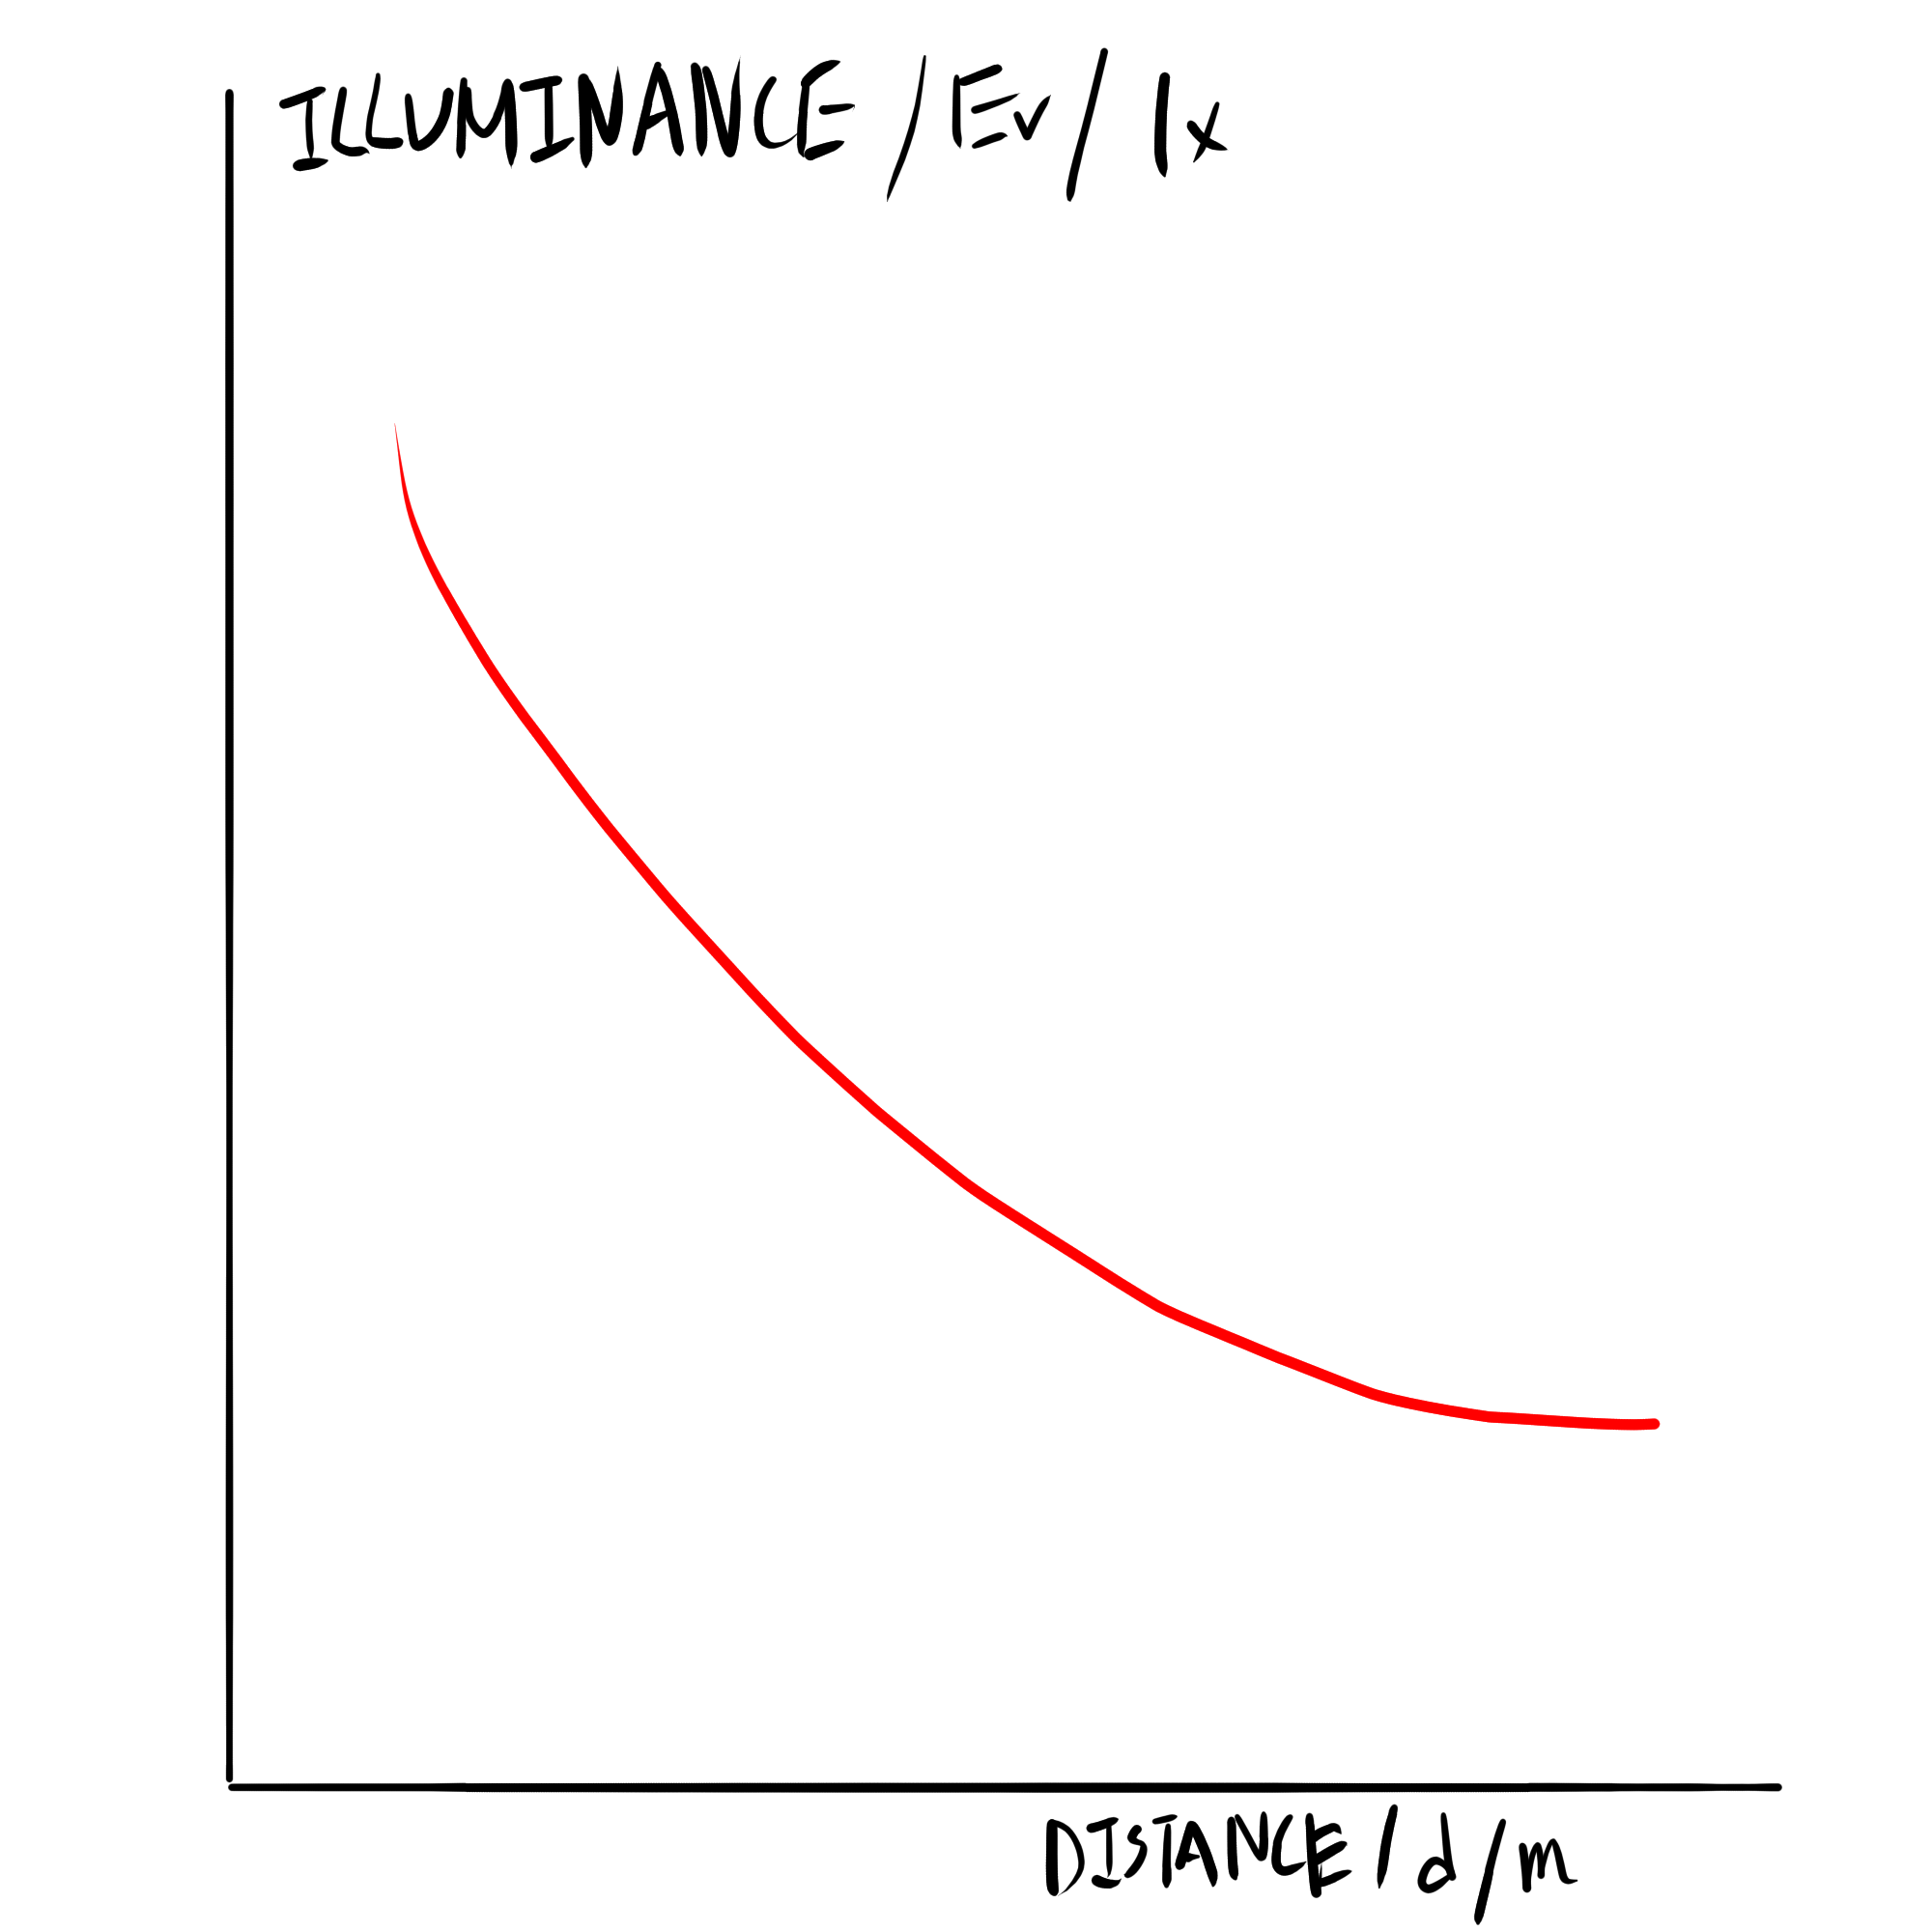
\includegraphics[width=0.37\textwidth]{assets/relationship.png}
    \caption{Graph of Illuminance against Distance}
    \label{fig:relation}
\end{figure}

The efficiency of the incandescent light-bulb can then be calculated using the proportionality constant $k$ of the illuminance vs. $1/\text{distance}^2$ relationship:

\[
E_v = k \frac{1}{d^2}
\]

The typical luminous efficacy $K$ of a light source is a measurement of the amount of light waves produced per watt, in unit $\frac{\si{lm}}{W}$. As the proportionality constant $k$ have unit $\si{lm}$, the typical luminous efficacy is the proportionality constant divided by the source power $P$:

\begin{figure}[H]
    \[
    K = \frac{k}{P}
    \]
    \caption{The typical luminous efficacy formula}
    \label{fig:tle}
\end{figure}


%However, the human eyes does not perceive the intensity of light uniformly through the wavelengths \parencite{candela}. Under conditions for photopic vision --- the vision of the eye in a well lit area, we perceive light in the green wavelength (555 $\si{nm}$) the most intensely. Therefore there is a need for a unit that displays the normalized intensity of different wavelengths of light --- the unit Candela and the photopic luminosity function \parencite{si_candela}.

% talk about the relationship between
%The intensity derived from the inverse square law (figure \ref{eq:isl}) is more formally known as the \textit{radiant intensity} \parencite{candela}, represented as a function of wavelength: $I_v(\lambda)$. By taking the incomplete integral on the weighted radiant intensity split into frequencies for all frequencies, we come to the definition of the \textit{luminous intensity} $I_v$, shown in figure \ref{eq:li}.

%\begin{figure}[h!]
%    \[
%     I_v = K_{cd} \int_{0}^{\infty} V(\lambda) %I_e(\lambda) \, d\lambda
%    \]
 %   \caption{The definition of Luminous Intensity}
 %   \label{eq:li}
%\end{figure}

%Combining the notion of luminous intensity with the 3D generalized angle quantity, steradian ($\si{\ohm}$), we can derive the total luminous power ($\Phi_v$) created by the source, measured in unit lumen ($\si{lm}$),

%\[
  %  \Phi_v = \si{\ohm} I_v,
%\]

%of which we can use to define the amount of luminous power incident on a surface through the quantity of illuminance, measured in units lux ($\si{lm\per m^2}$). The finalized relation is summarized in figure \ref{eq:dti}, \parencite{intensityLuminous_se}:

%\begin{figure}[h!]
% \centering
% \begin{align*}
% I_e(\lambda) &= c(\lambda) \frac{P}{4\pi s^2}\\
%  E_v &= \frac{1}{4\pi s^2 A} \si{\ohm} P K_{cd} \int_{0}^{\infty} V(\lambda) c(\lambda) \, d\lambda\\
%  E_v & \propto P\frac{1}{s^2}
% \end{align*}
% \caption{The complete distance to illuminance %relationship}
% \label{eq:dti}
%\end{figure}

%For the light sensor I have only measures intensity in lux, the above dive into luminosity serves as a justification for why I think the inverse square root applies to not just radiant intensity, but also to luminous intensity. Because the process of conversion is linear, it seems reasonable to hypothesize that illuminance is proportional to the distance squared.

% how to do it
To test the inverse square law, I decided to use a light sensor against a 5 watt light-bulb taken from the physics department. The light-bulb is supplied with only 8 volts out of the 12 volts power supply, as from past experience the bulb gets dangerously hot quickly on 12 volts. The dependent variable is the illuminance measurements from the light sensor, which ranges from 0-6000 lux. The independent variable is the distance of the light sensor from the light-bulb, ranging from 0.030m to 0.10m with steps of 0.01m, as this range provides a wide range of illuminance values from the specific light sensor. This is repeated for a total of 5 times because the light sensor often fluctuates even when held completely still. The repetition can help in reducing the uncertainties of the illuminance measurements.

%To test my hypothesis, I thought to conduct the experiment on the small 5W lab light-bulbs, for they have a tendency to heat up quickly before. Through some preliminary testing, I decided to decrease the supply voltage: the bulb gets dangerously hot on 12V, and placing sensor no closer than 3cm, and no further than 10cm, for at too close the illuminance exceeds the limits of the sensor, and that illuminance quickly drops off from the starting value, bringing no need of longer distances.

Additionally, I decided to connect a voltmeter along side an ammeter, because I have observed that the voltage provided by the supply always decreases when a component is connected to it. This is likely due to the internal resistance within the power supply. Therefore the voltmeter ensures a more accurate voltage measurement than the knob value on the power supply.

%This is to measure the power of the light source, but the voltmeter is significant in that I do not trust the supply voltage of the power supply. The power value can then be used to derive

\subsection{Variables}
\paragraph{Independent Variable}
The distance, measured in meters, the Vernier light sensor is from the 5W light-bulb.

\paragraph{Dependent Variable}
The illuminance of the area measured by the Vernier light sensor in unit lux.

\subsection{Control Variables}

\begin{longtable}{P{0.2\textwidth}|P{0.35\textwidth}|P{0.35\textwidth}}
Controls & Reason & How\\\hline
Ambient light intensity & Systematically increase the illuminance measurements from the light-bulb at all distances & Conduct the experiment in a dark location, and record the ambient illuminance of the room \\

The sensitivity of the light sensor & Light sensors are sensitive to angular tilts, and a disturbed sensor due to shaky hands most likely will produce random errors throughout the experiment & Use strong tape to clamp down the light sensor at the given distance\\

Fluctuation of the outside light intensity & Environmental lighting leaking through the lab windows fluctuating can randomly change the illuminance measurements at all distances & Conduct the experiment early in the morning, or late at night to minimize the effects from the sun \\

The power supplied to the light-bulb & A change in the supplied power will change measured illuminance at all distances, causing systematic errors & Assert the connected ammeter and voltmeter readings are unchanged after changing the independent variable, the distance\\

The temperature of the bulb filament & For the resistance of a resistor tends to increase at higher temperatures, the electrical current may decrease, decreasing the power supplied, creating systematic errors & It is best to conduct the experiment quickly --- in a span of an hour, as to minimize the extent of the heating of the light-bulb --- the physics light-bulbs heats up very quickly.

\end{longtable}

\newpage

\subsection{Materials}
\begin{itemize}
 \item Vernier light sensor ($\pm 2\si{lx}$) \parencite{vernier_manual} \& connection hub
 \item laptop with Vernier Data Logger software
 \item 5W light-bulb
 \item 12V power supply
 \item digital ammeter ($\pm 0.01\si{A}$) and voltmeter ($\pm 0.01\si{V}$)
 \item one meter long ruler ($\pm 0.001\si{m}$)
 \item duct tape
 \end{itemize}

\subsection{Method}

\begin{enumerate}
 \item Choose a location with the least amount of ambient light, preferably at a darkened room.

 \item Connect the Vernier light sensor to the laptop, set light sensor's range to (0–6000 \si{lx}). Enable ``Statistics'' in the Vernier logger lite software by clicking ``Stats''.

 \item Set up the electrical circuit as shown in diagram \ref{fig:cd}, set the power supply voltage to 8V, with a digital ammeter and voltmeter.

 \item Place the 1 meter ruler pointing towards the light-bulb, position the Vernier light sensor parallel to the ruler at a distance of 0.030m to the light-bulb. The final layout should be similar to figure \ref{fig:layout}.

 \item Secure down the light sensor at distances from 0.030m to 0.100m, step 0.010m, for a total of 8 distances.

 \item For each distance, record the readings on the ammeter and voltmeter, retry the measurement if they differ from the last distance. Record the illuminance over 10 seconds in the software, and note down the mean illuminance value as indicated in the software.

 \item Repeat steps 5-6 for a total of five times.
\end{enumerate}

\subsection{Diagrams}

% circuit
\begin{figure}[H]
\centering
\begin{circuitikz} \draw
    (0,3) to[battery,a=8V] (5,3) -- (5,0)
    to[lamp,a=5W] (0,0)
    to[rmeter, t=A] (0,3)
    (1,0) -- (1,-1.5)
    to[rmeter, t=V] (4,-1.5) -- (4,0)
    ;
\end{circuitikz}
\caption{The circuit diagram of the setup}
\label{fig:cd}
\end{figure}

% diagram
% annotated picture, & a software screen
\begin{figure}[H]
 \centering
 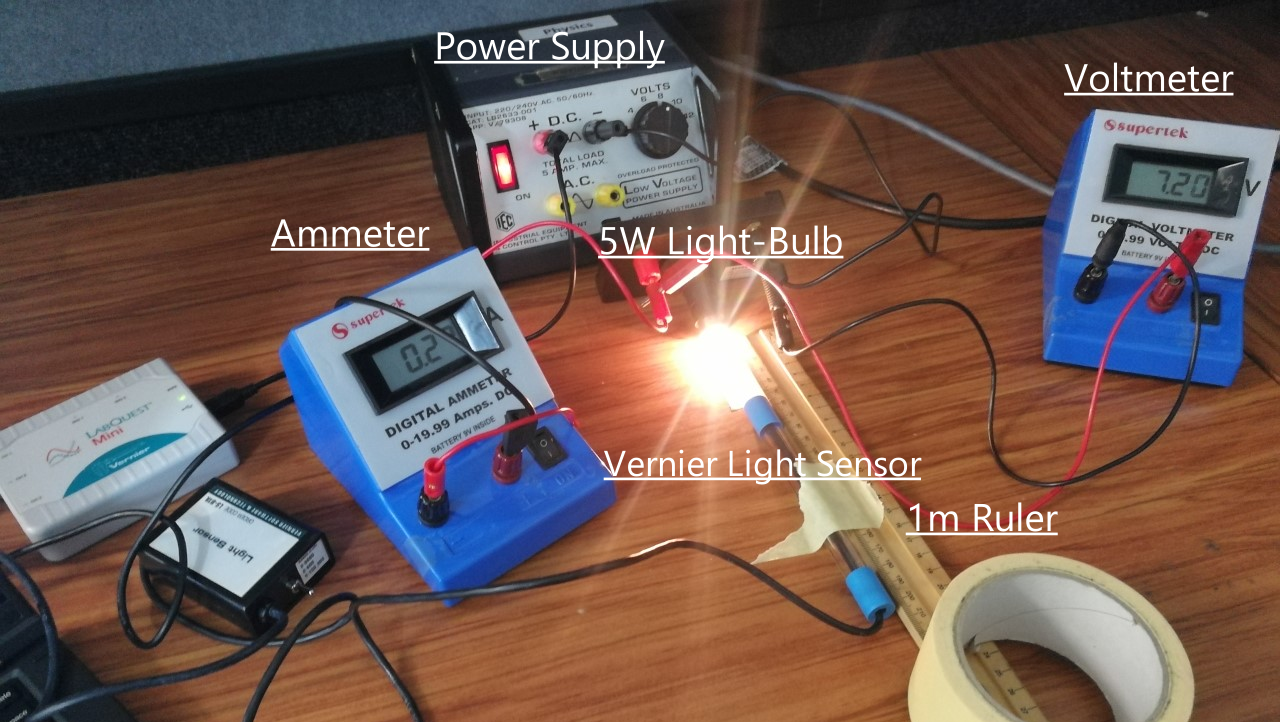
\includegraphics[width=\textwidth]{assets/setuppic.png}
 \caption{The experiment layout}
 \label{fig:layout}
\end{figure}


\subsection{Safety}
Avoid direct contact with exposed parts of the wires, additionally ensure a dry hand during the experiment. This will reduce the chance of an electrical accident.

Avoid touching the light-bulb throughout the experiment. The light-bulb got very hot during the experiment and direct skin contract may incur burns.

\section{Data}
\subsection{Raw data}
%\subsubsection*{Qualitative Data}
%As I conducted the experiment in a partially dark room, I noticed the ambient room light level occasionally changed in between the trials. I attempted to reduce this factor of error by setting up the experiment where my body was blocking the sun light.

%The screen light from my laptop had affected some initial measurements --- of which I had to re-measure. This led me to turn all devices off when measuring the illuminance values.

\subsubsection*{Quantitative Data}
\begin{figure}[H]
    \centering
    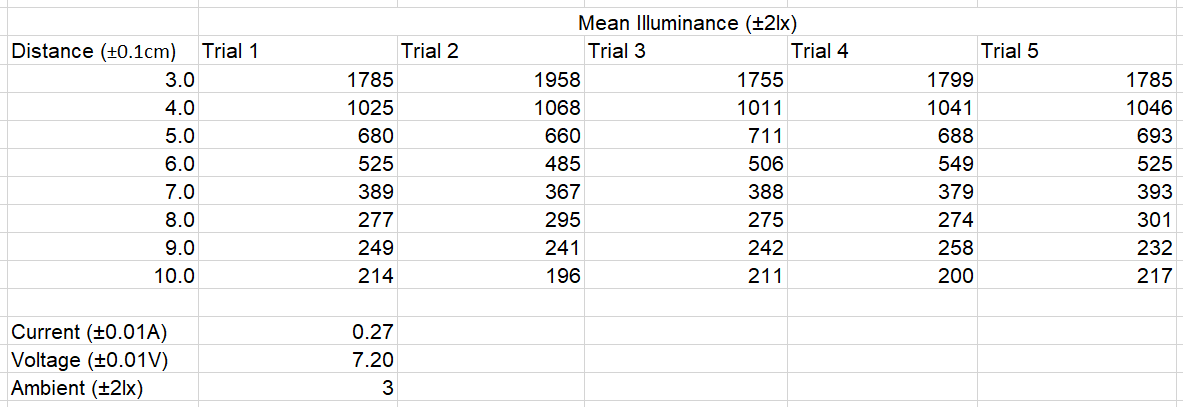
\includegraphics[width=\textwidth]{assets/rawdata.png}
    \caption{Raw quantitative experimental data}
    \label{fig:raw}
\end{figure}

\subsection{Processing}
\paragraph{Notation}

Uncertainty: unc, Absolute uncertainty: $\Delta$unc, Relative uncertainty: \%unc


\subsubsection{Processing Power}
The power is defined as the current times the voltage (figure \ref{eq:work}):
\begin{align*}
\text{Power} &= \text{Current} \times \text{Voltage}\\
        &= 0.27\si{A} \times 7.20\si{V} = 1.94 \si{W} \,(3 \tsf)
\end{align*}

\textit{Uncertainty of Power}: $\relun$Power =  $\relun$Current +  $\relun$Voltage
\begin{alignat*}{2}
    \% \text{unc}\, \si{I} &= \frac{0.01}{0.27} = 0.037,\quad &&\relun \si{V} = \frac{0.01}{7.20} = 0.0014\\
    \relun \si{W} &= 0.037 + 0.0014 = 0.04 \,(1 \tsf), \quad &&\absun \si{W} = 1.94 \times 0.04 = 0.08\si{W} \,(1 \tsf)
\end{alignat*}

Therefore: $\text{Power} = 1.94 \pm 0.08 \si{W}$

\subsubsection{Processing Illuminance}

\paragraphnl{Correcting for the ambient illuminance}
Subtract each illuminance values by the ambient illuminance value.

For example, in trial 1, at distance 0.030m:
\begin{align*}
    \text{Corrected} &= \text{Measured} - \text{Ambient }\\
    &= 1785 - 18 = 1767 \si{lx}
\end{align*}

\textit{Uncertainty of corrected illuminance}: $\absun$Corrected = $\absun$Measured + $\absun$Ambient
\begin{align*}
     \absun \text{Corrected} = 2 + 2 = 4\si{lx}
\end{align*}

%\begin{figure}[H]
 %   \centering
 %   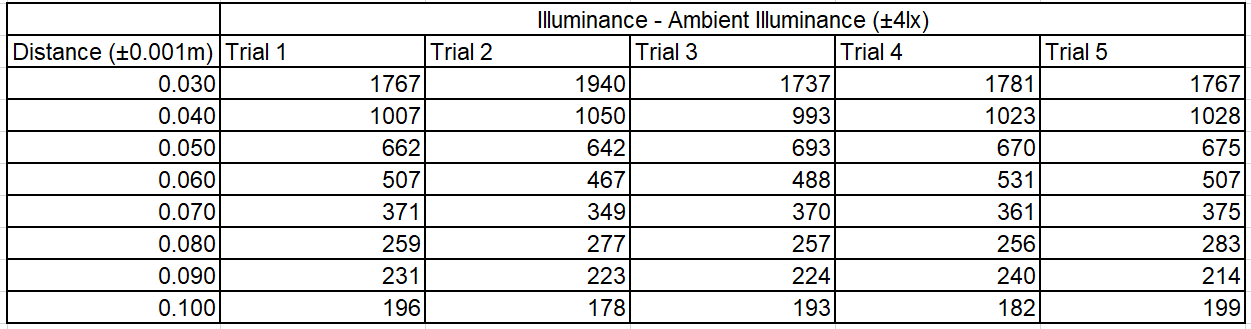
\includegraphics[scale=0.5]{assets/correcteddata.png}
 %   \caption{Corrected illuminance values}
 %   \label{fig:corrected}
%\end{figure}

\paragraphnl{Averaging trial illuminances}
Average the measured illuminance from 5 trials. Figure \ref{fig:average} shows the corrected illuminance values and the averages. Figure \ref{gph:average} plots the averaged illuminance values against the distances.

For example, averaging the illuminance measurements at distance 0.030m:
\begin{align*}
 \text{Illuminance}_{\text{average}} &= \frac{\sum \text{Illuminance}}{5}\\
 &= \frac{1767+1940+1737+1781+1767}{5}\\
 &= 1798\,\si{lx}
\end{align*}

\textit{Uncertainty using half ranges:} $\absun \text{Illum.}_{\text{average}} = \frac{\text{max}(\text{Illum}.) - \text{min}(\text{Illum}.)}{2}$

For example, at distance 0.030m:
\begin{align*}
 \absun \text{Illuminance}_{\text{average}} &= \frac{1940-1737}{2}\\
 &= 102 \,\si{lx}\\
 \text{Illuminance}_{\text{average}} &= 1800 \pm 100 \,\si{lx}
\end{align*}

\begin{figure}[H]
    \centering
    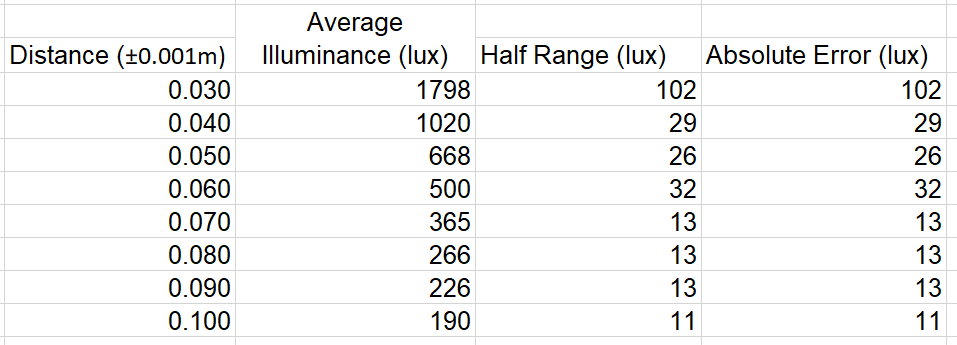
\includegraphics[width=\textwidth]{assets/averagedata.png}
    \caption{The averaged and corrected illuminance values}
    \label{fig:average}
\end{figure}

\begin{figure}[H]
    \centering
    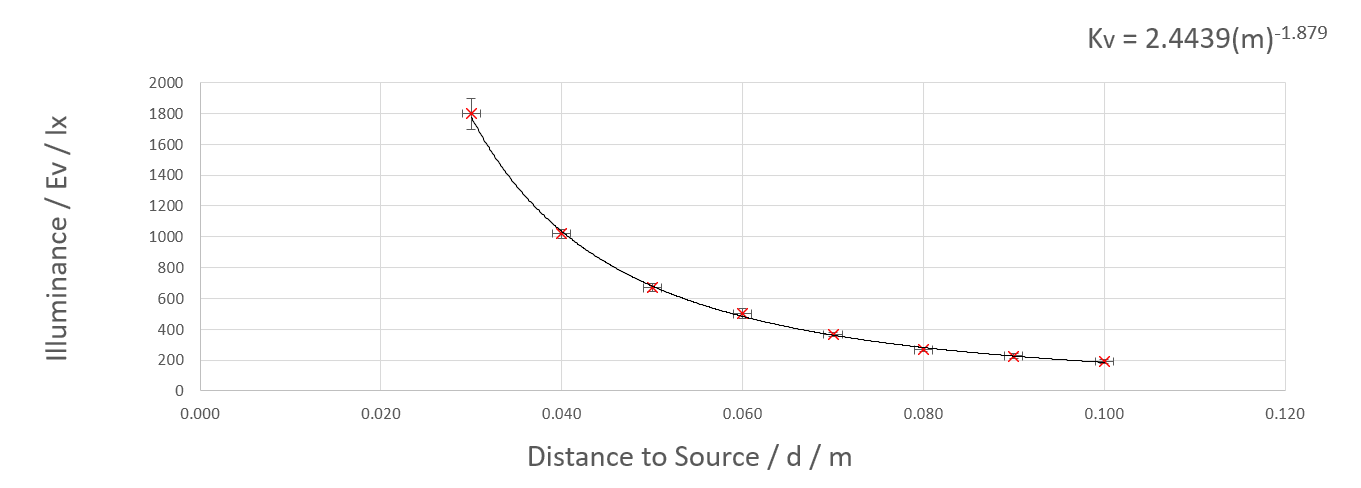
\includegraphics[width=\textwidth]{assets/averagegraph.png}
    \caption{Graph of the corrected and averaged illuminance values}
    \label{gph:average}
\end{figure}


\paragraphnl{Applying inverse squared transform on distance}
As figure \ref{gph:average} looks like an inverse squared graph, thus apply $1/{\text{distance}}^2$ transformation on the horizontal axis to straighten the graph. The transformation data and error is generated with Microsoft Excel (dataset: figure \ref{fig:tdata}, graph: figure \ref{gph:tdata}).

For example, at distance 0.030m:
\begin{align*}
 \frac{1}{\text{Distance}^2} &= 0.030 ^ {-2}\\
 &= 1110\,\si{m^{-2}}\, (3 \tsf)\\
\end{align*}

\textit{Uncertainty of the transformed distance}: $\relun 1/{\text{Distance}}^2$ = $2 \times \relun \text{Distance}$

For distance 0.030m:
\begin{align*}
 \relun 1/{\text{Distance}}^2 = 2 \times \relun \text{Distance} &= 2 \times 0.0333\\ &= 0.0667 \,(3 \tsf)\\
 \frac{1}{\text{Distance}^2} &= 1110\, \si{lx} \pm 6.67\%\\
 &= 1110 \pm 70 \,\si{lx}
\end{align*}


\begin{figure}[H]
    \centering
    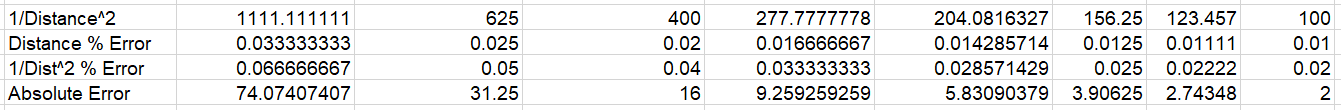
\includegraphics[width=\textwidth]{assets/transformdata.png}
    \caption{Transformed distance values and errors}
    \label{fig:tdata}
\end{figure}

\begin{figure}[H]
    \centering
    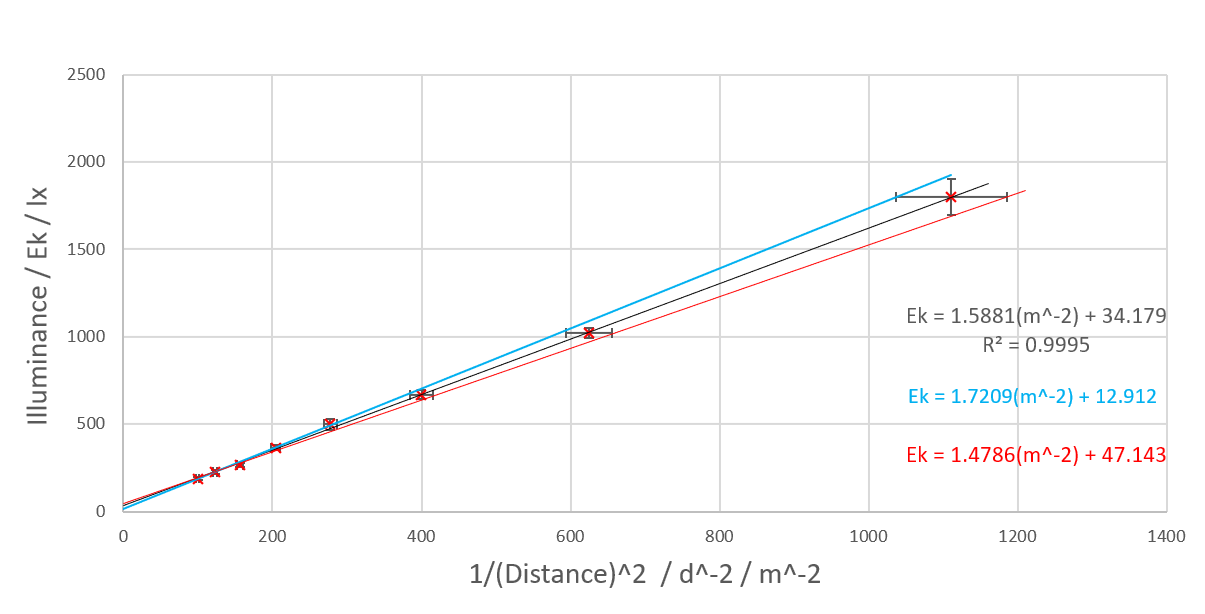
\includegraphics[width=\textwidth]{assets/transformgraph.png}
    \caption{Inverse squared distance to light source against the illuminance}
    \label{gph:tdata}
\end{figure}

\paragraphnl{Gradient and Errors}
Figure \ref{gph:tdata} also displays the regression line and its equation (top equation), and the two lines of worst fits for error calculations (middle and lower equation). The $1/\text{Distance}^2$ horizontal error bars are used for plotting the line of worst fits as they are larger in size then the illuminance/vertical errors. The uncertainty of the gradient and y-intercept of the regression line are calculated using the half range of values in the line of worst fits.

%The justification for the horizontal error line of worst fits in figure \ref{gph:tdata} resides in the accuracy of the measuring devices: the percentage errors of the ruler are (for all values) larger than the percentage error of the light sensor, as indicated by the size of the error bars.

Regression line gradient, y-intercept: 1.59, 34.2 ($3 \tsf$)

\textit{Uncertainty of gradient using half range}:\\
Highest gradient error line gradient, y-intercept: 1.72, 12.9 ($3 \tsf$).

Lowest gradient error line gradient, y-intercept: 1.48, 47.1 ($3 \tsf$).

Gradient uncertainty: $\frac{1.72-1.48}{2} = 0.120$

y-intercept uncertainty: $\frac{47.1-12.9}{2} = 17.1$

Therefore, the regression line and thus the relationship between illuminance $E_v$ against the distance $d$ is:

%Therefore, the relationship is summarized as in figure \ref{fig:rel}:
\begin{figure}[h!]
    \[
       E_v = (1.6 \pm 0.1) \frac{1}{d^2} + (30 \pm 20)
    \]
    \caption{Experimental relationship between illuminance against distance from source}
    \label{fig:rel}
\end{figure}

% TODO: compare with actual data

\section{Conclusions}
\subsection{Result}

There exists a clear and strong inverse squared relationship between the illuminance and the distance to the light-bulb, as shown in the transformed graph in figure \ref{gph:tdata}, and the close to one correlation coefficient $\sqrt{0.9995}=0.9997$. This shows that as the distance to a light source increases, the illuminance decreases relatively rapidly at close distances but relatively less at far distances, and vice versa.
%Following the data collection and some transformation for linearization, the relationship is summarized in figure \ref{fig:rel}. The data had mostly supported the theory of the inverse square law. From figure \ref{gph:average}, one can see the that the measured illuminance falls rapidly when the distance to source increases. To create a linear curve, the illuminance ($E_v$) is plotted against the inverse square of the distance ($\frac{1}{d^2}$) shown in figure \ref{gph:tdata}. The small variance of the data points from the regression line is a strong evidence to support my hypothesis.

However, the theory of inverse square law also suggests that the relationship curve should have a y-intercept of 0. The non-zero y-intercept of the regression line --- even considering the ranges of uncertainty ($0 \notin [10, 50]$), suggests some systematical errors are present. The curve is shifted upwards by a sizable amount, which could be caused by the erroneous reading of the ambient illuminance, parallax error in aligning the ruler, or by a lack of calibration of the light sensor. This indicates that the experiment data was not very accurate.

The graph (figure \ref{gph:tdata}) consists of noticeable sized error bars that increases as distance increases. This is caused by the small distances used in combination with the moderately uncertain wooden ruler used. However the results are overall relatively precise due to the low percentage uncertainty of the two axis (figure \ref{fig:tdata}, figure \ref{fig:average}). The experiment data is considered to be precise but inaccurate.

%TODO: maybe include this, or not
%The high correlation coefficient showcases the strong inverse squared relationship between the distance to the light source and the illuminance. This is because light waves from a light source radiates outwards in a perfect sphere, with surface area inversely proportional to the distance to its origin squared. As light intensity is measured in power per area, the larger the sphere surface area, the less intensity of the light as the amount of light waves spreads out. This means that the light intensity is also inversely proportional to the distance squared.

%Additionally, the experimental data contains a noticeable amount of uncertainties indicated by the large error bars, particularly at smaller distances. There also exists large random error in the illuminance measurement, as indicated by the high half ranges of the trials of illuminance measurements during averaging (figure \ref{fig:average}) --- sometimes to a degree of $102/1798 \approx 5.7\%$ at the distance of $3\si{cm}$. This is most likely caused by the fluctuation of the light level in the room, which is likely caused by the leakage of sunlight through the window blinds. This is also reflected in the gradient calculations, for the slope had a relatively large uncertainty of $12.1\%$, supporting the presence of large random errors. However, the averaging of the data seemed to reduce the effects of the error. The line of best fit passed through all 8 points of the independent variable, and had a very high R-squared value of $0.9995$ and R value of $\sqrt{0.9995} \approx 0.9997$. This shows a high level of correlation in the data. In conclusion, the raw dataset presented in figure \ref{fig:raw} is said to be highly accuracy but less precise, and contains medium amounts of uncertainty.

\subsection{Implications}

%If we were to define the proportionality constant $\eta$ in figure \ref{eq:li} with parameter power, such that:

%\begin{align*}
%    \eta &= \frac{1}{4\pi A} \si{\ohm} K_{cd} \int_{0}^{\infty} V(\lambda) c(\lambda) \, d\lambda\\
 %   E_v &= \eta P \frac{1}{s^2},
%\end{align*}

%where $\eta$ is another constant, I can fulfill my motivation for this experiment. Notice the units of the constant $\eta$ is $(\frac{\si{lx}}{\si{W\per m^2}} = \frac{\si{lm}}{\si{W}})$, is a value that is only depended on the light source used. Therefore, the constant $\eta$ is a measure of the efficacy of the light-bulb used in the amount of luminous power produced per unit power. This is also known as the typical luminous efficacy, one that I can use to compare to other light-bulbs using an online database. Furthermore, the value can be used to compare efficiency of light-bulbs in your daily life, whether that is to save money, or like me, to appreciate how far lighting technology had advanced.

The typical luminous efficacy $K$ can be calculated by dividing the gradient constant $k$ by the power dissipated $P$ (figure \ref{fig:tle}):
%A division is needed to calculate the luminous efficacy $\eta$:
\begin{align*}
    K &= \frac{k}{P} = \frac{1.6 \pm 0.1}{1.94 \pm 0.07}\\
    &= 0.82 \pm 0.08\,\si{lm\per W}\,(2\, \tsf)
\end{align*}

\begin{wrapfigure}{r}{0.45\textwidth}
    \centering
    \begin{tabular}{l|l}
        Category     & Luminous Efficacy (lm/W) \\ \hline
        Combustion   & 1-2                      \\
        Incandescent & 5-17.5                   \\
        Halogen      & 16.7-35                  \\
        Fluorescent  & 46-104.2                 \\
        LED          & 75-210
    \end{tabular}
    \caption{List of common luminous efficacy values of light sources\protect\footnotemark}
    \label{tbl:leff}
\end{wrapfigure}

\footnotetext{ \parencite{le_value1} \parencite{le_value2}  \parencite{le_value3} \parencite{le_value4}}


Comparing to the luminous efficacy values of a set of common light sources in figure \ref{tbl:leff}, the physics lab incandescent 5W light-bulb with a luminous efficacy value of $0.82 (\si{lm\per W})$, looks to be as efficient in producing light as a typical fireplace. This is unsurprising, as the outer glass casing of the bulb readily heats up when it is powered, indicating energy loss in the form of thermal energy. A suggestion is to made for the school physics department for a switch to safer (less glass temperature), and more energy efficient light-bulbs for general experiments.

\subsection{Reflection}

Here is a list on the handling of the controlled variables/potential error factors, and future improvements to be made.

\subsubsection{Random Errors}
\paragraph{Fluctuation of the outside light level} This is potentially a significant factor in creating a large uncertainty and low precision in the raw illuminance data. The advice would be to conduct the experiment at night, or in a totally blackout room without light pollution. This will increase the precision of the experiment and decrease the uncertainty on the luminous efficacy.

\paragraph{The sensitivity of the light sensor} Insignificant, for the equipment is properly taped down, removing the problem of a shaky hand.

\paragraph{The power supplied to the light-bulb}
Insignificant, for the power held stable during the experiment.

\subsubsection{Systematic Errors}
\paragraph{Environmental room intensity}
A potentially significant variable. The small but existent systematic error is likely to be caused by the erroneous measure of the ambient room light level. Performing the experiment in a blackout room or at night is likely to reduce the effects of the ambient room intensity and increase the accuracy of the dataset, possibility creating a curve that intercepts closer to 0 on the y axis.

\paragraph{The temperature of the bulb filament}
Insignificant, for the power is kept below the operating power limit and a lack of systematic decreasing illuminance during trials.

\paragraph{Parallax placements of the ruler}
A potentially significant variable. For the wooden ruler have depth, an angled top-down view to place the ruler is likely to result in parallax errors, thus systematically displacing the measured distances. It may be wise to have used a paper with beforehand markings of the distances, which is likely in reducing the systematic error shown in the curve, and potentially help bring the intercept closer to point (0,0).

\paragraph{Accuracy of the light sensor}
A variable that I was the most concerned about. This may be the largest cause of the systematic error. I could follow a lengthy calibration test listed on the manufacture's website against a factory calibrated source, which will decrease the systematic error and increase the accuracy of the data.

\subsection{Further Investigations}
Consider repeating the experiment with several other household lighting sources --- LED, halogen, or fluorescent light-bulbs, and compare their typical luminous efficacy. The information can be used to determine the efficiency of different types of light sources to help the physics department to choose more efficient light-bulbs.

%\nocite{*}
\newpage
\printbibliography



\end{document}
